\documentclass{article} % Starts an article
\usepackage{amsmath}
\usepackage{graphicx}
\usepackage{listings}
\usepackage{amsfonts}
\graphicspath{ {./} }
\author{Alexis}
\title{Queen Attack} % Title

\begin{document} % Begins a document
  \maketitle

  \section{Problem Statement}

  Consider a 2D square grid of size $N$. $N$ queens are assigned a color in $1, ..., C$. $W$ Walls are also placed on static cells.

  Walls ($-1$), empty cells ($0$) and queens ($1, ..., C$) are identified using a 2D integer array $color[N][N]$. The values range from $-1$ to $C$.

  \begin{figure}[h]
    \centering
    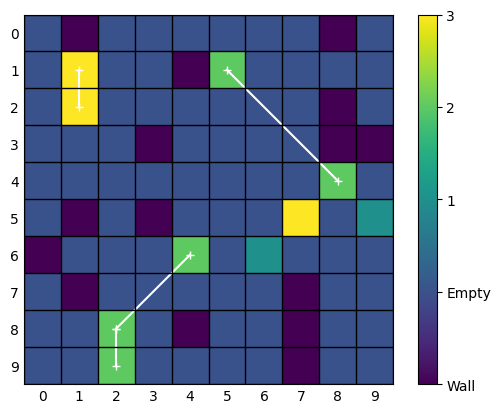
\includegraphics{QueenAttackBoard}
    \caption{The number of pairs under attack is $0 (1) + 3 (2) + 1 (3) = 4$}
    \label{fig:QueenAttackBoard}
  \end{figure}

  Consider all the pairs of same-color queens under attack of each others. One can move a queen to avoid being under attack. The goal is to minimize the overall cost

  \[ min \{ attackCost + moveCost \} \]

  \section{Attack cost}

  The \textit{attack} cost is the sum of attack pairs weighted by a factor $N$

  \[ attackCost = N * attackPairs \]

  The number of pairs of queens under attack with the same color

  \[ attackPairs = \sum_{(x_1, y_1) | color[x_1, y_1] > 0} attackPairs(x_1, y_1) \]

  For a queen at position $(x_1, y_1)$ with color $c$, the number of other queens under attack without double counting is

  \begin{align*}
      attackPairs(x_1, y_1) & = attackDown(x_1, y_1) \\
                               & + attackRight(x_1, y_1) \\
                               & + attackDownLeft(x_1, y_1) \\
                               & + attackDownRight(x_1, y_1)
  \end{align*}

  $attackDown$, $attackRight$, $attackDownLeft$ or $attackDownRight$ is a boolean. With
  
  \[ c = color[x_1, y_1 ]\]
  
  It is true if the closest non-empty cell in associated direction is also a queen with color $c$. 

  \begin{align*}
    attackDown(x_1, y_1)      & \Leftarrow color[x_1+k_d, y_1]           &= c \\
    attackRight(x_1, y_1)     & \Leftarrow color[x_1, y_1+k_r]           &= c \\
    attackDownLeft(x_1, y_1)  & \Leftarrow color[x_1+k_{dl}, y_1-k_{dl}] &= c \\
    attackDownRight(x_1, y_1) & \Leftarrow color[x_1+k_{dr}, y_1+k_{dr}] &= c
  \end{align*}

  \subsection{Neighbors}

  \begin{figure}[h]
    \centering
    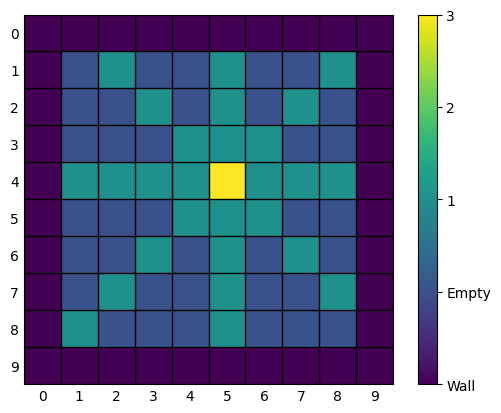
\includegraphics{QueenAttackPairs}
    \caption{Positions under attack by the queen at $(x_1, y_1) = (4, 5)$}
    \label{fig:QueenAttackPairs}
  \end{figure}

  \begin{table}
    \centering
    \begin{tabular}{|c|c|}
      \hline
      \textbf{Direction} & $(x_2, y_2)$ \\
      \hline
      Down & $(x_1+k_d, y_1)$\\
      \hline
      Right & $(x_1, y_1+k_r)$\\
      \hline
      Down-Left & $(x_1+k_{dl}, y_1-k_{dl})$\\
      \hline
      Down-Right & $(x_1+k_{dr}, y_1+k_{dr})$ \\
      \hline
      Up & $(x_1-k_u, y_1)$\\
      \hline
      Left & $(x_1, y_1-k_l)$\\
      \hline
      Up-Left & $(x_1-k_{ul}, y_1-k_{ul})$\\
      \hline
      Up-Right & $(x_1-k_{ur}, y_1+k_{ur})$ \\
      \hline
    \end{tabular}
    \caption{Position $(x_2, y_2)$ for the 2nd queen under attack by the 1st queen at position $(x_1, y_1)$}
    \label{tab:QueenAttackDirections}
  \end{table}

  Where is the closest non-empty cell from $(x_1, y_1)$ in every direction ? It is the min offset to a non-empty cell. By inserting walls all around the grid we ensure such neighbors always exist.

  \begin{align*}
    k_d = min \{ k \in \mathbb{N} & | k > 0 \\
                                  &   x_2 = x_1+k < N \\
                                  &   y_2 = y_1
                                  &   color[x_2, y_2] \ne 0 \}
  \end{align*}

  \begin{align*}
    k_r = min \{ k \in \mathbb{N} & | k > 0 \\
                                  &   x_2 = x_1
                                  &   y_2 = y_1+k < N \\
                                  &   color[x_2, y_2] \ne 0 \}
  \end{align*}

  \begin{align*}
    k_{dl} = min \{ k \in \mathbb{N} & | k > 0 \\
                                    &   x_2 = x_1+k < N \\
                                    &   y_2 = y_1-k >= 0 \\
                                    &   color[x_2, y_2] \ne 0 \}
  \end{align*}

  \begin{align*}
    k_{dr} = min \{ k \in \mathbb{N} & | k > 0 \\
                                    &   x_2 = x_1+k < N \\
                                    &   y_2 = y_1+k < N \\
                                    &   color[x_2, y_2] \ne 0 \}
  \end{align*}

  \begin{align*}
    k_u = min \{ k \in \mathbb{N} & | k > 0 \\
                                  &   x_2 = x_1-k >= 0 \\
                                  &   y_2 = y_1 \\
                                  &   color[x_2, y_2] \ne 0 \}
  \end{align*}

  \begin{align*}
    k_l = min \{ k \in \mathbb{N} & | k > 0 \\
                                  &   x_2 = x_1 \\
                                  &   y_2 = y_1-k >= 0 \\
                                  &   color[x_2, y_2] \ne 0 \}
  \end{align*}

  \begin{align*}
    k_{ul} = min \{ k \in \mathbb{N} & | k > 0 \\
                                     &   x_2 = x_1-k >= 0 \\
                                     &   y_2 - y_1-k >= 0 \\
                                     &   color[x_2, y_2] \ne 0 \}
  \end{align*}

  \begin{align*}
    k_{ur} = min \{ k \in \mathbb{N} & | k > 0 \\
                                     &   x_2 = x_1-k >= 0 \\
                                     &   y_2 = y_1+k < N \\
                                     &   color[x_2, y_2] \ne 0 \}
  \end{align*}


  \section{Move cost}

  One generates a sequence of moves to reduce the \textit{attack} cost.

  A queen can move horizontally, vertically or diagonally as long as the move is valid: no other queens or walls are blocking the move.
  
  At each time $t \in {1, ..., T}$, one chooses 1. a queen on the chess board located at position $(x_{1}, y_{1})$ and 2. an empty cell at position $(x_{2}, y_{2})$ to move it to.

  \begin{align*}
    color[x_2,y_2] &= 0 \\
    color[x_1,y_1] &> 0
  \end{align*}
  
  Given $(x_1,y_1)$, consider $k_d, k_r, k_{dl}, k_{dr}, k_u, k_l, k_{ul}, k_{ur}$ the offsets to the neighbor positions. The new position $(x_2,y_2)$ and the \textit{move} offset $k>0$ verify one of the constraints in Table \ref{tab:QueenAttackMove}. This incurs into a \textit{move} cost of

  \[ moveCost_t = \sqrt{max\{|x_{2}-x_{1}|, |y_{2}-y_{1}|\}} = \sqrt{k} \]

  \begin{table}
    \centering
    \begin{tabular}{|c|c|c|}
      \hline
      \textbf{Direction} & $x_2$ & $y_2$ \\
      \hline
      Down & $x_1 + k < x_1 + k_d$ & $y_1$ \\
      \hline
      Right & $x_1$ & $y_1 + k < y_1 + k_r$ \\
      \hline
      Down-Left & $x_1 + k < x_1 + k_{dl}$ & $y_1 - k > y_1 - k_{dl}$ \\
      \hline
      Down-Right & $x_1 + k < x_1 + k_{dr}$ & $y_1 + k < y_1 + k_{dr}$ \\
      \hline
      Up & $x_1 - k > x_1 - k_u$ & $y_1$ \\
      \hline
      Left & $x_1$ & $y_1 - k > y_1 - k_l$ \\
      \hline
      Up-Left & $x_1 - k > x_1 - k_{ul}$ & $y_1 - k > y_1 - k_{ul}$ \\
      \hline
      Up-Right & $x_1 - k > x_1 - k_{ur}$ & $y_1 + k < y_1 + k_{ur}$ \\
      \hline
    \end{tabular}
    \caption{Offset $k$ and position $(x_2, y_2)$ for the queen move from position $(x_1, y_1)$}
    \label{tab:QueenAttackMove}
  \end{table}
  
  The sequence \textit{move} cost is the sum of the cost of each moves

  \[ moveCost = \sum_{t=1}^{T} moveCost_t \]

  If one decides to make a move, the state is updated to

  \begin{align*}
    color[x_2,y_2] &= color[x_1,y_1] \\
    color[x_1,y_1] &= 0
  \end{align*}

  \end{document}